\begin{appendix}

\chapter{Anhang}

\section{Die Algorithmen}

\subsection{Programmablaufplan der Algorithmen}

\begin{figure}
  \centering
      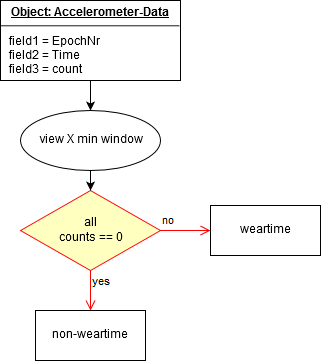
\includegraphics[width=0.5\textwidth]{Bilder/naiver_ansatz.png}
    \caption{\ naiv}
    \label{flow:naiv}
\end{figure}

\begin{figure}
  \centering
      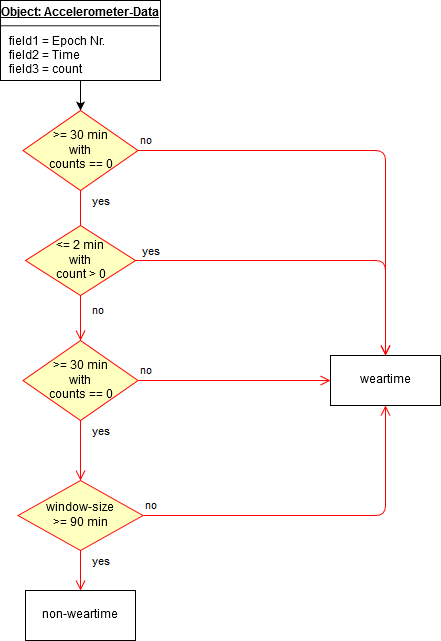
\includegraphics[width=0.5\textwidth]{Bilder/Choi.png}
    \caption{\ Choi}
    \label{flow:choi}
\end{figure}

\begin{figure}
  \centering
      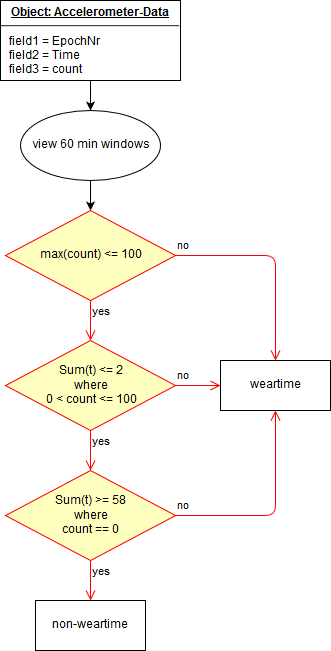
\includegraphics[width=0.5\textwidth]{Bilder/Troiano.png}
    \caption{\ Troiano}
    \label{flow:troiano}
\end{figure}

\begin{figure}
  \centering
      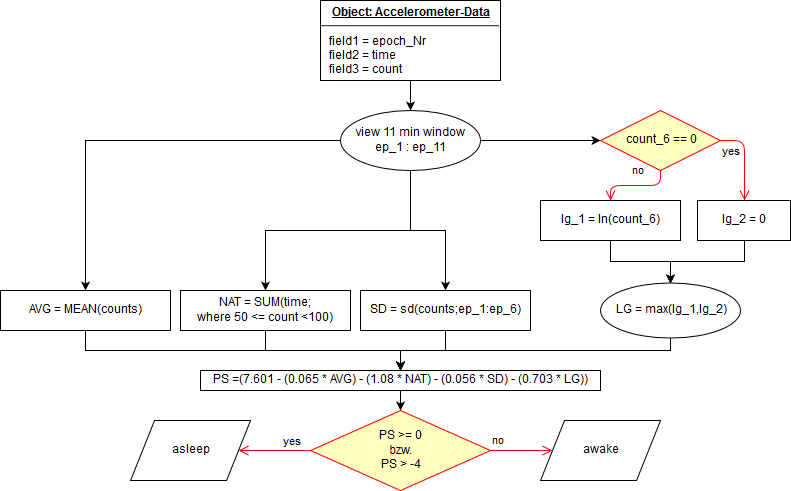
\includegraphics[width=0.5\textwidth]{Bilder/slp_sadeh.png}
    \caption{\ sadeh}
    \label{flow:sadeh}
\end{figure}

\begin{figure}
  \centering
      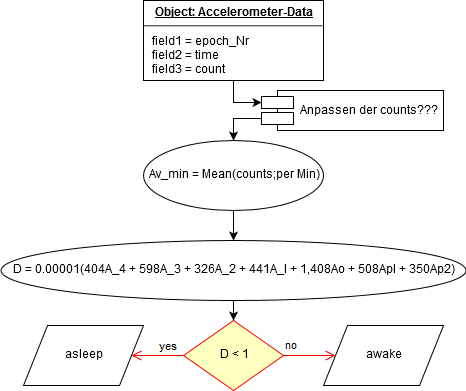
\includegraphics[width=0.5\textwidth]{Bilder/cole-kripke.png}
    \caption{\ Cole-Kripke}
    \label{flow:cole}
\end{figure}

\subsection{Visualisierung der Algorithmen des maschinellen lernens}



\section{Fragebögen}


\section{...}


\end{appendix}
%\backmatter